\documentclass[1p]{elsarticle_modified}
%\bibliographystyle{elsarticle-num}

%\usepackage[colorlinks]{hyperref}
%\usepackage{abbrmath_seonhwa} %\Abb, \Ascr, \Acal ,\Abf, \Afrak
\usepackage{amsfonts}
\usepackage{amssymb}
\usepackage{amsmath}
\usepackage{amsthm}
\usepackage{scalefnt}
\usepackage{amsbsy}
\usepackage{kotex}
\usepackage{caption}
\usepackage{subfig}
\usepackage{color}
\usepackage{graphicx}
\usepackage{xcolor} %% white, black, red, green, blue, cyan, magenta, yellow
\usepackage{float}
\usepackage{setspace}
\usepackage{hyperref}

\usepackage{tikz}
\usetikzlibrary{arrows}

\usepackage{multirow}
\usepackage{array} % fixed length table
\usepackage{hhline}

%%%%%%%%%%%%%%%%%%%%%
\makeatletter
\renewcommand*\env@matrix[1][\arraystretch]{%
	\edef\arraystretch{#1}%
	\hskip -\arraycolsep
	\let\@ifnextchar\new@ifnextchar
	\array{*\c@MaxMatrixCols c}}
\makeatother %https://tex.stackexchange.com/questions/14071/how-can-i-increase-the-line-spacing-in-a-matrix
%%%%%%%%%%%%%%%

\usepackage[normalem]{ulem}

\newcommand{\msout}[1]{\ifmmode\text{\sout{\ensuremath{#1}}}\else\sout{#1}\fi}
%SOURCE: \msout is \stkout macro in https://tex.stackexchange.com/questions/20609/strikeout-in-math-mode

\newcommand{\cancel}[1]{
	\ifmmode
	{\color{red}\msout{#1}}
	\else
	{\color{red}\sout{#1}}
	\fi
}

\newcommand{\add}[1]{
	{\color{blue}\uwave{#1}}
}

\newcommand{\replace}[2]{
	\ifmmode
	{\color{red}\msout{#1}}{\color{blue}\uwave{#2}}
	\else
	{\color{red}\sout{#1}}{\color{blue}\uwave{#2}}
	\fi
}

\newcommand{\Sol}{\mathcal{S}} %segment
\newcommand{\D}{D} %diagram
\newcommand{\A}{\mathcal{A}} %arc


%%%%%%%%%%%%%%%%%%%%%%%%%%%%%5 test

\def\sl{\operatorname{\textup{SL}}(2,\Cbb)}
\def\psl{\operatorname{\textup{PSL}}(2,\Cbb)}
\def\quan{\mkern 1mu \triangleright \mkern 1mu}

\theoremstyle{definition}
\newtheorem{thm}{Theorem}[section]
\newtheorem{prop}[thm]{Proposition}
\newtheorem{lem}[thm]{Lemma}
\newtheorem{ques}[thm]{Question}
\newtheorem{cor}[thm]{Corollary}
\newtheorem{defn}[thm]{Definition}
\newtheorem{exam}[thm]{Example}
\newtheorem{rmk}[thm]{Remark}
\newtheorem{alg}[thm]{Algorithm}

\newcommand{\I}{\sqrt{-1}}
\begin{document}

%\begin{frontmatter}
%
%\title{Boundary parabolic representations of knots up to 8 crossings}
%
%%% Group authors per affiliation:
%\author{Yunhi Cho} 
%\address{Department of Mathematics, University of Seoul, Seoul, Korea}
%\ead{yhcho@uos.ac.kr}
%
%
%\author{Seonhwa Kim} %\fnref{s_kim}}
%\address{Center for Geometry and Physics, Institute for Basic Science, Pohang, 37673, Korea}
%\ead{ryeona17@ibs.re.kr}
%
%\author{Hyuk Kim}
%\address{Department of Mathematical Sciences, Seoul National University, Seoul 08826, Korea}
%\ead{hyukkim@snu.ac.kr}
%
%\author{Seokbeom Yoon}
%\address{Department of Mathematical Sciences, Seoul National University, Seoul, 08826,  Korea}
%\ead{sbyoon15@snu.ac.kr}
%
%\begin{abstract}
%We find all boundary parabolic representation of knots up to 8 crossings.
%
%\end{abstract}
%\begin{keyword}
%    \MSC[2010] 57M25 
%\end{keyword}
%
%\end{frontmatter}

%\linenumbers
%\tableofcontents
%
\newcommand\colored[1]{\textcolor{white}{\rule[-0.35ex]{0.8em}{1.4ex}}\kern-0.8em\color{red} #1}%
%\newcommand\colored[1]{\textcolor{white}{ #1}\kern-2.17ex	\textcolor{white}{ #1}\kern-1.81ex	\textcolor{white}{ #1}\kern-2.15ex\color{red}#1	}

{\Large $\underline{12n_{0125}~(K12n_{0125})}$}

\setlength{\tabcolsep}{10pt}
\renewcommand{\arraystretch}{1.6}
\vspace{1cm}\begin{tabular}{m{100pt}>{\centering\arraybackslash}m{274pt}}
\multirow{5}{120pt}{
	\centering
	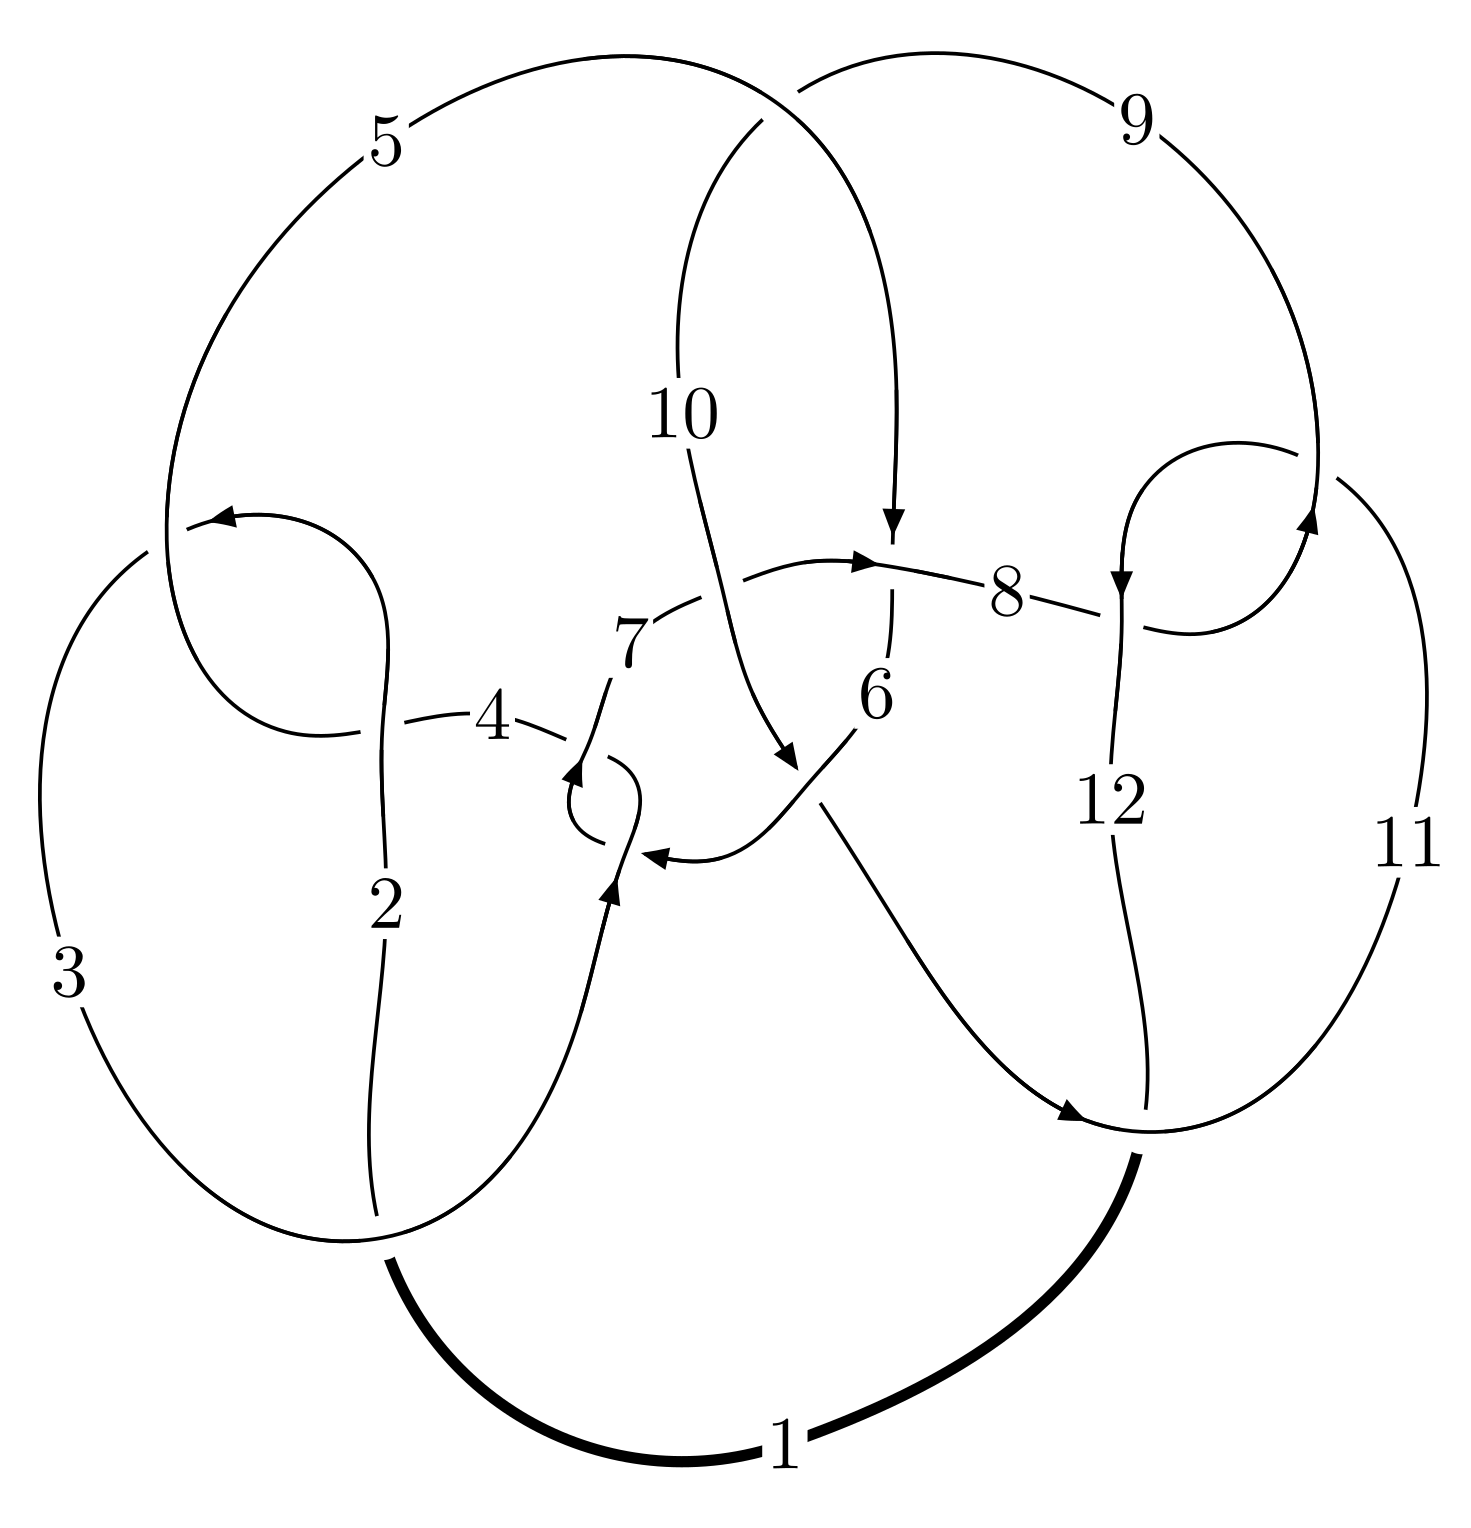
\includegraphics[width=112pt]{../../../GIT/diagram.site/Diagrams/png/2214_12n_0125.png}\\
\ \ \ A knot diagram\footnotemark}&
\allowdisplaybreaks
\textbf{Linearized knot diagam} \\
\cline{2-2}
 &
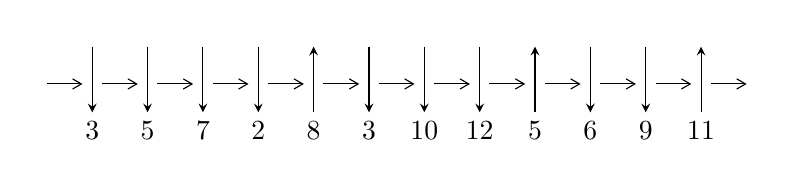
\begin{tikzpicture}[x=20pt, y=17pt]
	% nodes
	\node (C0) at (0, 0) {};
	\node (C1) at (1, 0) {};
	\node (C1U) at (1, +1) {};
	\node (C1D) at (1, -1) {3};

	\node (C2) at (2, 0) {};
	\node (C2U) at (2, +1) {};
	\node (C2D) at (2, -1) {5};

	\node (C3) at (3, 0) {};
	\node (C3U) at (3, +1) {};
	\node (C3D) at (3, -1) {7};

	\node (C4) at (4, 0) {};
	\node (C4U) at (4, +1) {};
	\node (C4D) at (4, -1) {2};

	\node (C5) at (5, 0) {};
	\node (C5U) at (5, +1) {};
	\node (C5D) at (5, -1) {8};

	\node (C6) at (6, 0) {};
	\node (C6U) at (6, +1) {};
	\node (C6D) at (6, -1) {3};

	\node (C7) at (7, 0) {};
	\node (C7U) at (7, +1) {};
	\node (C7D) at (7, -1) {10};

	\node (C8) at (8, 0) {};
	\node (C8U) at (8, +1) {};
	\node (C8D) at (8, -1) {12};

	\node (C9) at (9, 0) {};
	\node (C9U) at (9, +1) {};
	\node (C9D) at (9, -1) {5};

	\node (C10) at (10, 0) {};
	\node (C10U) at (10, +1) {};
	\node (C10D) at (10, -1) {6};

	\node (C11) at (11, 0) {};
	\node (C11U) at (11, +1) {};
	\node (C11D) at (11, -1) {9};

	\node (C12) at (12, 0) {};
	\node (C12U) at (12, +1) {};
	\node (C12D) at (12, -1) {11};
	\node (C13) at (13, 0) {};

	% arrows
	\draw[->,>={angle 60}]
	(C0) edge (C1) (C1) edge (C2) (C2) edge (C3) (C3) edge (C4) (C4) edge (C5) (C5) edge (C6) (C6) edge (C7) (C7) edge (C8) (C8) edge (C9) (C9) edge (C10) (C10) edge (C11) (C11) edge (C12) (C12) edge (C13) ;	\draw[->,>=stealth]
	(C1U) edge (C1D) (C2U) edge (C2D) (C3U) edge (C3D) (C4U) edge (C4D) (C5D) edge (C5U) (C6U) edge (C6D) (C7U) edge (C7D) (C8U) edge (C8D) (C9D) edge (C9U) (C10U) edge (C10D) (C11U) edge (C11D) (C12D) edge (C12U) ;
	\end{tikzpicture} \\
\hhline{~~} \\& 
\textbf{Solving Sequence} \\ \cline{2-2} 
 &
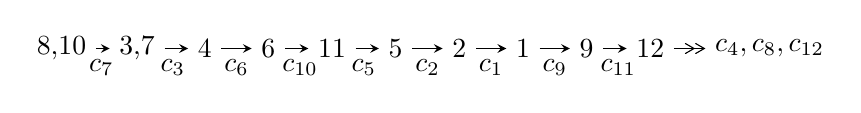
\begin{tikzpicture}[x=23pt, y=7pt]
	% node
	\node (A0) at (-1/8, 0) {8,10};
	\node (A1) at (17/16, 0) {3,7};
	\node (A2) at (17/8, 0) {4};
	\node (A3) at (25/8, 0) {6};
	\node (A4) at (33/8, 0) {11};
	\node (A5) at (41/8, 0) {5};
	\node (A6) at (49/8, 0) {2};
	\node (A7) at (57/8, 0) {1};
	\node (A8) at (65/8, 0) {9};
	\node (A9) at (73/8, 0) {12};
	\node (C1) at (1/2, -1) {$c_{7}$};
	\node (C2) at (13/8, -1) {$c_{3}$};
	\node (C3) at (21/8, -1) {$c_{6}$};
	\node (C4) at (29/8, -1) {$c_{10}$};
	\node (C5) at (37/8, -1) {$c_{5}$};
	\node (C6) at (45/8, -1) {$c_{2}$};
	\node (C7) at (53/8, -1) {$c_{1}$};
	\node (C8) at (61/8, -1) {$c_{9}$};
	\node (C9) at (69/8, -1) {$c_{11}$};
	\node (A10) at (11, 0) {$c_{4},c_{8},c_{12}$};

	% edge
	\draw[->,>=stealth]	
	(A0) edge (A1) (A1) edge (A2) (A2) edge (A3) (A3) edge (A4) (A4) edge (A5) (A5) edge (A6) (A6) edge (A7) (A7) edge (A8) (A8) edge (A9) ;
	\draw[->>,>={angle 60}]	
	(A9) edge (A10);
\end{tikzpicture} \\ 

\end{tabular} \\

\footnotetext{
The image of knot diagram is generated by the software ``\textbf{Draw programme}" developed by Andrew Bartholomew(\url{http://www.layer8.co.uk/maths/draw/index.htm\#Running-draw}), where we modified some parts for our purpose(\url{https://github.com/CATsTAILs/LinksPainter}).
}\phantom \\ \newline 
\centering \textbf{Ideals for irreducible components\footnotemark of $X_{\text{par}}$} 
 
\begin{align*}
I^u_{1}&=\langle 
-5.24906\times10^{251} u^{61}-2.63379\times10^{252} u^{60}+\cdots+3.44441\times10^{254} b+2.69575\times10^{254},\\
\phantom{I^u_{1}}&\phantom{= \langle  }1.32614\times10^{254} u^{61}+8.14465\times10^{254} u^{60}+\cdots+2.75553\times10^{255} a+1.08450\times10^{257},\\
\phantom{I^u_{1}}&\phantom{= \langle  }u^{62}+6 u^{61}+\cdots+1248 u+64\rangle \\
I^u_{2}&=\langle 
- u^3- u^2+b- u,\;- u^3+a+2,\;u^4+u^2- u+1\rangle \\
I^u_{3}&=\langle 
2 u^5+u^4+3 u^3+2 u^2+b+2 u+2,\;-2 u^5-4 u^3- u^2+a-3 u-2,\;u^6+u^5+2 u^4+2 u^3+2 u^2+2 u+1\rangle \\
\\
I^v_{1}&=\langle 
a,\;186 v^5+1767 v^4+16759 v^3+279 v^2+385 b+93 v+306,\;v^6+10 v^5+95 v^4+48 v^3+15 v^2+5 v+1\rangle \\
\end{align*}
\raggedright * 4 irreducible components of $\dim_{\mathbb{C}}=0$, with total 78 representations.\\
\footnotetext{All coefficients of polynomials are rational numbers. But the coefficients are sometimes approximated in decimal forms when there is not enough margin.}
\newpage
\renewcommand{\arraystretch}{1}
\centering \section*{I. $I^u_{1}= \langle -5.25\times10^{251} u^{61}-2.63\times10^{252} u^{60}+\cdots+3.44\times10^{254} b+2.70\times10^{254},\;1.33\times10^{254} u^{61}+8.14\times10^{254} u^{60}+\cdots+2.76\times10^{255} a+1.08\times10^{257},\;u^{62}+6 u^{61}+\cdots+1248 u+64 \rangle$}
\flushleft \textbf{(i) Arc colorings}\\
\begin{tabular}{m{7pt} m{180pt} m{7pt} m{180pt} }
\flushright $a_{8}=$&$\begin{pmatrix}1\\0\end{pmatrix}$ \\
\flushright $a_{10}=$&$\begin{pmatrix}0\\u\end{pmatrix}$ \\
\flushright $a_{3}=$&$\begin{pmatrix}-0.0481264 u^{61}-0.295575 u^{60}+\cdots-637.661 u-39.3574\\0.00152394 u^{61}+0.00764656 u^{60}+\cdots-7.07240 u-0.782645\end{pmatrix}$ \\
\flushright $a_{7}=$&$\begin{pmatrix}1\\- u^2\end{pmatrix}$ \\
\flushright $a_{4}=$&$\begin{pmatrix}-0.0507184 u^{61}-0.309962 u^{60}+\cdots-642.175 u-39.0110\\0.00177774 u^{61}+0.00929252 u^{60}+\cdots-5.78492 u-0.708113\end{pmatrix}$ \\
\flushright $a_{6}=$&$\begin{pmatrix}-0.0290606 u^{61}-0.178730 u^{60}+\cdots-379.788 u-22.2184\\0.000355637 u^{61}+0.000276515 u^{60}+\cdots-9.59505 u-0.781127\end{pmatrix}$ \\
\flushright $a_{11}=$&$\begin{pmatrix}0.165545 u^{61}+0.979872 u^{60}+\cdots+380.906 u-1.53739\\0.00433759 u^{61}+0.0238765 u^{60}+\cdots+4.60076 u+0.0296773\end{pmatrix}$ \\
\flushright $a_{5}=$&$\begin{pmatrix}-0.0294163 u^{61}-0.179007 u^{60}+\cdots-370.193 u-21.4373\\0.000355637 u^{61}+0.000276515 u^{60}+\cdots-9.59505 u-0.781127\end{pmatrix}$ \\
\flushright $a_{2}=$&$\begin{pmatrix}-0.0294071 u^{61}-0.179875 u^{60}+\cdots-373.738 u-23.7994\\-0.000269202 u^{61}-0.00331814 u^{60}+\cdots-10.7470 u-0.840234\end{pmatrix}$ \\
\flushright $a_{1}=$&$\begin{pmatrix}-0.00835458 u^{61}-0.0484189 u^{60}+\cdots-50.9506 u-3.17945\\- u^2\end{pmatrix}$ \\
\flushright $a_{9}=$&$\begin{pmatrix}0.160433 u^{61}+0.951245 u^{60}+\cdots+378.382 u-1.35204\\0.000774875 u^{61}+0.00475004 u^{60}+\cdots-0.0771139 u-0.215021\end{pmatrix}$ \\
\flushright $a_{12}=$&$\begin{pmatrix}0.0505800 u^{61}+0.275509 u^{60}+\cdots-864.856 u-57.5492\\0.00229093 u^{61}+0.0128560 u^{60}+\cdots-5.13956 u-0.334034\end{pmatrix}$\\&\end{tabular}
\flushleft \textbf{(ii) Obstruction class $= -1$}\\~\\
\flushleft \textbf{(iii) Cusp Shapes $= -0.134110 u^{61}-0.834494 u^{60}+\cdots-2032.73 u-106.916$}\\~\\
\newpage\renewcommand{\arraystretch}{1}
\flushleft \textbf{(iv) u-Polynomials at the component}\newline \\
\begin{tabular}{m{50pt}|m{274pt}}
Crossings & \hspace{64pt}u-Polynomials at each crossing \\
\hline $$\begin{aligned}c_{1}\end{aligned}$$&$\begin{aligned}
&u^{62}+71 u^{61}+\cdots+267 u+1
\end{aligned}$\\
\hline $$\begin{aligned}c_{2},c_{4}\end{aligned}$$&$\begin{aligned}
&u^{62}-13 u^{61}+\cdots+15 u-1
\end{aligned}$\\
\hline $$\begin{aligned}c_{3},c_{6}\end{aligned}$$&$\begin{aligned}
&u^{62}+3 u^{61}+\cdots-8192 u-1024
\end{aligned}$\\
\hline $$\begin{aligned}c_{5}\end{aligned}$$&$\begin{aligned}
&u^{62}+4 u^{61}+\cdots-10 u^2+1
\end{aligned}$\\
\hline $$\begin{aligned}c_{7}\end{aligned}$$&$\begin{aligned}
&u^{62}-6 u^{61}+\cdots-1248 u+64
\end{aligned}$\\
\hline $$\begin{aligned}c_{8},c_{11}\end{aligned}$$&$\begin{aligned}
&u^{62}-5 u^{61}+\cdots+113 u+1
\end{aligned}$\\
\hline $$\begin{aligned}c_{9}\end{aligned}$$&$\begin{aligned}
&u^{62}+44 u^{60}+\cdots+9664 u+824
\end{aligned}$\\
\hline $$\begin{aligned}c_{10}\end{aligned}$$&$\begin{aligned}
&u^{62}+4 u^{61}+\cdots-3025807 u+537503
\end{aligned}$\\
\hline $$\begin{aligned}c_{12}\end{aligned}$$&$\begin{aligned}
&u^{62}-21 u^{61}+\cdots+12769 u+1
\end{aligned}$\\
\hline
\end{tabular}\\~\\
\newpage\renewcommand{\arraystretch}{1}
\flushleft \textbf{(v) Riley Polynomials at the component}\newline \\
\begin{tabular}{m{50pt}|m{274pt}}
Crossings & \hspace{64pt}Riley Polynomials at each crossing \\
\hline $$\begin{aligned}c_{1}\end{aligned}$$&$\begin{aligned}
&y^{62}-147 y^{61}+\cdots-20183 y+1
\end{aligned}$\\
\hline $$\begin{aligned}c_{2},c_{4}\end{aligned}$$&$\begin{aligned}
&y^{62}-71 y^{61}+\cdots-267 y+1
\end{aligned}$\\
\hline $$\begin{aligned}c_{3},c_{6}\end{aligned}$$&$\begin{aligned}
&y^{62}-57 y^{61}+\cdots+9961472 y+1048576
\end{aligned}$\\
\hline $$\begin{aligned}c_{5}\end{aligned}$$&$\begin{aligned}
&y^{62}-4 y^{61}+\cdots-20 y+1
\end{aligned}$\\
\hline $$\begin{aligned}c_{7}\end{aligned}$$&$\begin{aligned}
&y^{62}-30 y^{61}+\cdots-185344 y+4096
\end{aligned}$\\
\hline $$\begin{aligned}c_{8},c_{11}\end{aligned}$$&$\begin{aligned}
&y^{62}+21 y^{61}+\cdots-12769 y+1
\end{aligned}$\\
\hline $$\begin{aligned}c_{9}\end{aligned}$$&$\begin{aligned}
&y^{62}+88 y^{61}+\cdots+13013520 y+678976
\end{aligned}$\\
\hline $$\begin{aligned}c_{10}\end{aligned}$$&$\begin{aligned}
&y^{62}+16 y^{61}+\cdots-11200434939731 y+288909475009
\end{aligned}$\\
\hline $$\begin{aligned}c_{12}\end{aligned}$$&$\begin{aligned}
&y^{62}+45 y^{61}+\cdots-163345321 y+1
\end{aligned}$\\
\hline
\end{tabular}\\~\\
\newpage\flushleft \textbf{(vi) Complex Volumes and Cusp Shapes}
$$\begin{array}{c|c|c}  
\text{Solutions to }I^u_{1}& \I (\text{vol} + \sqrt{-1}CS) & \text{Cusp shape}\\
 \hline 
\begin{aligned}
u &= -0.966330\phantom{ +0.000000I} \\
a &= \phantom{-}2.06084\phantom{ +0.000000I} \\
b &= -0.132404\phantom{ +0.000000I}\end{aligned}
 & -10.3258\phantom{ +0.000000I} & -5.46580\phantom{ +0.000000I} \\ \hline\begin{aligned}
u &= \phantom{-}0.225473 + 1.012430 I \\
a &= \phantom{-}0.68800 - 2.63426 I \\
b &= -0.10147 - 2.38732 I\end{aligned}
 & -2.91907 - 1.90864 I & -12.3927 + 9.8412 I \\ \hline\begin{aligned}
u &= \phantom{-}0.225473 - 1.012430 I \\
a &= \phantom{-}0.68800 + 2.63426 I \\
b &= -0.10147 + 2.38732 I\end{aligned}
 & -2.91907 + 1.90864 I & -12.3927 - 9.8412 I \\ \hline\begin{aligned}
u &= \phantom{-}0.906197 + 0.566629 I \\
a &= \phantom{-}0.898820 - 1.059170 I \\
b &= -0.080489 - 0.151302 I\end{aligned}
 & -6.85055 - 2.44704 I & \phantom{-0.000000 } 0 \\ \hline\begin{aligned}
u &= \phantom{-}0.906197 - 0.566629 I \\
a &= \phantom{-}0.898820 + 1.059170 I \\
b &= -0.080489 + 0.151302 I\end{aligned}
 & -6.85055 + 2.44704 I & \phantom{-0.000000 } 0 \\ \hline\begin{aligned}
u &= \phantom{-}0.630967 + 0.873245 I \\
a &= -0.0480953 + 0.0962373 I \\
b &= \phantom{-}0.066678 - 0.565097 I\end{aligned}
 & -0.54827 - 2.57263 I & \phantom{-0.000000 } 0 \\ \hline\begin{aligned}
u &= \phantom{-}0.630967 - 0.873245 I \\
a &= -0.0480953 - 0.0962373 I \\
b &= \phantom{-}0.066678 + 0.565097 I\end{aligned}
 & -0.54827 + 2.57263 I & \phantom{-0.000000 } 0 \\ \hline\begin{aligned}
u &= -0.428788 + 0.808171 I \\
a &= \phantom{-}0.166658 + 0.166436 I \\
b &= \phantom{-}0.144316 + 0.950356 I\end{aligned}
 & \phantom{-}3.58947 + 0.62301 I & \phantom{-}3.36345 - 2.22600 I \\ \hline\begin{aligned}
u &= -0.428788 - 0.808171 I \\
a &= \phantom{-}0.166658 - 0.166436 I \\
b &= \phantom{-}0.144316 - 0.950356 I\end{aligned}
 & \phantom{-}3.58947 - 0.62301 I & \phantom{-}3.36345 + 2.22600 I \\ \hline\begin{aligned}
u &= \phantom{-}0.175720 + 0.877651 I \\
a &= -1.87346 - 0.71678 I \\
b &= \phantom{-}0.1068970 - 0.0427277 I\end{aligned}
 & -9.63287 + 2.57588 I & -1.03891 + 4.65048 I\\
 \hline 
 \end{array}$$\newpage$$\begin{array}{c|c|c}  
\text{Solutions to }I^u_{1}& \I (\text{vol} + \sqrt{-1}CS) & \text{Cusp shape}\\
 \hline 
\begin{aligned}
u &= \phantom{-}0.175720 - 0.877651 I \\
a &= -1.87346 + 0.71678 I \\
b &= \phantom{-}0.1068970 + 0.0427277 I\end{aligned}
 & -9.63287 - 2.57588 I & -1.03891 - 4.65048 I \\ \hline\begin{aligned}
u &= -0.613756 + 1.022410 I \\
a &= -0.0631222 + 0.0157113 I \\
b &= -0.017254 + 0.535087 I\end{aligned}
 & \phantom{-}1.46847 + 7.47551 I & \phantom{-0.000000 } 0 \\ \hline\begin{aligned}
u &= -0.613756 - 1.022410 I \\
a &= -0.0631222 - 0.0157113 I \\
b &= -0.017254 - 0.535087 I\end{aligned}
 & \phantom{-}1.46847 - 7.47551 I & \phantom{-0.000000 } 0 \\ \hline\begin{aligned}
u &= \phantom{-}1.148340 + 0.333874 I \\
a &= \phantom{-}1.27542 + 0.77535 I \\
b &= -0.26412 - 2.34055 I\end{aligned}
 & -3.40045 - 1.02073 I & \phantom{-0.000000 } 0 \\ \hline\begin{aligned}
u &= \phantom{-}1.148340 - 0.333874 I \\
a &= \phantom{-}1.27542 - 0.77535 I \\
b &= -0.26412 + 2.34055 I\end{aligned}
 & -3.40045 + 1.02073 I & \phantom{-0.000000 } 0 \\ \hline\begin{aligned}
u &= -0.768297 + 0.223225 I \\
a &= -1.92583 + 0.47346 I \\
b &= \phantom{-}0.61700 - 1.55498 I\end{aligned}
 & -0.90689 + 2.60619 I & -4.21909 - 1.98730 I \\ \hline\begin{aligned}
u &= -0.768297 - 0.223225 I \\
a &= -1.92583 - 0.47346 I \\
b &= \phantom{-}0.61700 + 1.55498 I\end{aligned}
 & -0.90689 - 2.60619 I & -4.21909 + 1.98730 I \\ \hline\begin{aligned}
u &= -0.625920 + 0.391100 I \\
a &= \phantom{-}1.359350 - 0.293081 I \\
b &= -0.217590 + 0.449117 I\end{aligned}
 & \phantom{-}0.16449 - 2.80931 I & -2.02619 + 2.03045 I \\ \hline\begin{aligned}
u &= -0.625920 - 0.391100 I \\
a &= \phantom{-}1.359350 + 0.293081 I \\
b &= -0.217590 - 0.449117 I\end{aligned}
 & \phantom{-}0.16449 + 2.80931 I & -2.02619 - 2.03045 I \\ \hline\begin{aligned}
u &= -0.569996 + 0.465415 I \\
a &= -2.68911 - 0.37051 I \\
b &= -0.345079 - 0.969509 I\end{aligned}
 & -0.271555 + 0.561550 I & -5.56822 - 2.77116 I\\
 \hline 
 \end{array}$$\newpage$$\begin{array}{c|c|c}  
\text{Solutions to }I^u_{1}& \I (\text{vol} + \sqrt{-1}CS) & \text{Cusp shape}\\
 \hline 
\begin{aligned}
u &= -0.569996 - 0.465415 I \\
a &= -2.68911 + 0.37051 I \\
b &= -0.345079 + 0.969509 I\end{aligned}
 & -0.271555 - 0.561550 I & -5.56822 + 2.77116 I \\ \hline\begin{aligned}
u &= \phantom{-}1.269210 + 0.022101 I \\
a &= -1.118240 - 0.162406 I \\
b &= \phantom{-}0.125530 + 0.806401 I\end{aligned}
 & -5.71401 + 2.41800 I & \phantom{-0.000000 } 0 \\ \hline\begin{aligned}
u &= \phantom{-}1.269210 - 0.022101 I \\
a &= -1.118240 + 0.162406 I \\
b &= \phantom{-}0.125530 - 0.806401 I\end{aligned}
 & -5.71401 - 2.41800 I & \phantom{-0.000000 } 0 \\ \hline\begin{aligned}
u &= -1.268290 + 0.189716 I \\
a &= -1.227750 + 0.054676 I \\
b &= \phantom{-}0.107949 - 0.868842 I\end{aligned}
 & -5.53536 + 3.45054 I & \phantom{-0.000000 } 0 \\ \hline\begin{aligned}
u &= -1.268290 - 0.189716 I \\
a &= -1.227750 - 0.054676 I \\
b &= \phantom{-}0.107949 + 0.868842 I\end{aligned}
 & -5.53536 - 3.45054 I & \phantom{-0.000000 } 0 \\ \hline\begin{aligned}
u &= -1.187220 + 0.502909 I \\
a &= \phantom{-}1.52617 - 0.01474 I \\
b &= -0.80672 + 1.64220 I\end{aligned}
 & \phantom{-}1.17723 + 4.19224 I & \phantom{-0.000000 } 0 \\ \hline\begin{aligned}
u &= -1.187220 - 0.502909 I \\
a &= \phantom{-}1.52617 + 0.01474 I \\
b &= -0.80672 - 1.64220 I\end{aligned}
 & \phantom{-}1.17723 - 4.19224 I & \phantom{-0.000000 } 0 \\ \hline\begin{aligned}
u &= \phantom{-}0.568930 + 0.416577 I \\
a &= \phantom{-}0.120281 + 1.074160 I \\
b &= \phantom{-}0.045387 - 0.507767 I\end{aligned}
 & -0.76460 - 1.25688 I & -5.53847 + 5.17379 I \\ \hline\begin{aligned}
u &= \phantom{-}0.568930 - 0.416577 I \\
a &= \phantom{-}0.120281 - 1.074160 I \\
b &= \phantom{-}0.045387 + 0.507767 I\end{aligned}
 & -0.76460 + 1.25688 I & -5.53847 - 5.17379 I \\ \hline\begin{aligned}
u &= -0.453256 + 1.217240 I \\
a &= \phantom{-}0.90351 + 1.13576 I \\
b &= \phantom{-}0.71700 + 2.26803 I\end{aligned}
 & -2.25042 - 3.70807 I & \phantom{-0.000000 } 0\\
 \hline 
 \end{array}$$\newpage$$\begin{array}{c|c|c}  
\text{Solutions to }I^u_{1}& \I (\text{vol} + \sqrt{-1}CS) & \text{Cusp shape}\\
 \hline 
\begin{aligned}
u &= -0.453256 - 1.217240 I \\
a &= \phantom{-}0.90351 - 1.13576 I \\
b &= \phantom{-}0.71700 - 2.26803 I\end{aligned}
 & -2.25042 + 3.70807 I & \phantom{-0.000000 } 0 \\ \hline\begin{aligned}
u &= -0.042454 + 0.695928 I \\
a &= -0.025549 + 0.219032 I \\
b &= -0.276487 + 1.114370 I\end{aligned}
 & \phantom{-}3.47148 + 0.76506 I & \phantom{-}5.05392 - 1.67806 I \\ \hline\begin{aligned}
u &= -0.042454 - 0.695928 I \\
a &= -0.025549 - 0.219032 I \\
b &= -0.276487 - 1.114370 I\end{aligned}
 & \phantom{-}3.47148 - 0.76506 I & \phantom{-}5.05392 + 1.67806 I \\ \hline\begin{aligned}
u &= \phantom{-}0.384833 + 0.475726 I \\
a &= \phantom{-}1.82484 + 0.76996 I \\
b &= -0.016778 - 0.470642 I\end{aligned}
 & -0.75966 - 1.41499 I & -4.04897 + 4.67258 I \\ \hline\begin{aligned}
u &= \phantom{-}0.384833 - 0.475726 I \\
a &= \phantom{-}1.82484 - 0.76996 I \\
b &= -0.016778 + 0.470642 I\end{aligned}
 & -0.75966 + 1.41499 I & -4.04897 - 4.67258 I \\ \hline\begin{aligned}
u &= -1.33070 + 0.53202 I \\
a &= \phantom{-}1.058240 + 0.373107 I \\
b &= -0.234697 + 0.167699 I\end{aligned}
 & -13.75470 + 2.34725 I & \phantom{-0.000000 } 0 \\ \hline\begin{aligned}
u &= -1.33070 - 0.53202 I \\
a &= \phantom{-}1.058240 - 0.373107 I \\
b &= -0.234697 - 0.167699 I\end{aligned}
 & -13.75470 - 2.34725 I & \phantom{-0.000000 } 0 \\ \hline\begin{aligned}
u &= -0.468299 + 0.280082 I \\
a &= -0.059976 - 0.302032 I \\
b &= -0.276860 - 1.385290 I\end{aligned}
 & \phantom{-}2.81830 - 4.57708 I & -11.91750 - 5.21602 I \\ \hline\begin{aligned}
u &= -0.468299 - 0.280082 I \\
a &= -0.059976 + 0.302032 I \\
b &= -0.276860 + 1.385290 I\end{aligned}
 & \phantom{-}2.81830 + 4.57708 I & -11.91750 + 5.21602 I \\ \hline\begin{aligned}
u &= \phantom{-}1.30977 + 0.65145 I \\
a &= \phantom{-}0.967015 - 0.381842 I \\
b &= -0.229472 - 0.212903 I\end{aligned}
 & -12.7715 - 8.3839 I & \phantom{-0.000000 } 0\\
 \hline 
 \end{array}$$\newpage$$\begin{array}{c|c|c}  
\text{Solutions to }I^u_{1}& \I (\text{vol} + \sqrt{-1}CS) & \text{Cusp shape}\\
 \hline 
\begin{aligned}
u &= \phantom{-}1.30977 - 0.65145 I \\
a &= \phantom{-}0.967015 + 0.381842 I \\
b &= -0.229472 + 0.212903 I\end{aligned}
 & -12.7715 + 8.3839 I & \phantom{-0.000000 } 0 \\ \hline\begin{aligned}
u &= \phantom{-}1.43373 + 0.32544 I \\
a &= \phantom{-}0.1365400 - 0.0114578 I \\
b &= -0.05979 + 1.64995 I\end{aligned}
 & -8.50399 - 1.01711 I & \phantom{-0.000000 } 0 \\ \hline\begin{aligned}
u &= \phantom{-}1.43373 - 0.32544 I \\
a &= \phantom{-}0.1365400 + 0.0114578 I \\
b &= -0.05979 - 1.64995 I\end{aligned}
 & -8.50399 + 1.01711 I & \phantom{-0.000000 } 0 \\ \hline\begin{aligned}
u &= -1.40066 + 0.45878 I \\
a &= \phantom{-}0.0626733 - 0.1057400 I \\
b &= -0.04777 - 1.57885 I\end{aligned}
 & -7.87011 + 7.16358 I & \phantom{-0.000000 } 0 \\ \hline\begin{aligned}
u &= -1.40066 - 0.45878 I \\
a &= \phantom{-}0.0626733 + 0.1057400 I \\
b &= -0.04777 + 1.57885 I\end{aligned}
 & -7.87011 - 7.16358 I & \phantom{-0.000000 } 0 \\ \hline\begin{aligned}
u &= \phantom{-}1.39279 + 0.63989 I \\
a &= \phantom{-}1.172420 - 0.173984 I \\
b &= -0.44372 - 1.75238 I\end{aligned}
 & -6.43547 - 4.60616 I & \phantom{-0.000000 } 0 \\ \hline\begin{aligned}
u &= \phantom{-}1.39279 - 0.63989 I \\
a &= \phantom{-}1.172420 + 0.173984 I \\
b &= -0.44372 + 1.75238 I\end{aligned}
 & -6.43547 + 4.60616 I & \phantom{-0.000000 } 0 \\ \hline\begin{aligned}
u &= -1.35459 + 0.72187 I \\
a &= \phantom{-}1.220540 + 0.275631 I \\
b &= -0.42983 + 1.70660 I\end{aligned}
 & -5.32588 + 10.75820 I & \phantom{-0.000000 } 0 \\ \hline\begin{aligned}
u &= -1.35459 - 0.72187 I \\
a &= \phantom{-}1.220540 - 0.275631 I \\
b &= -0.42983 - 1.70660 I\end{aligned}
 & -5.32588 - 10.75820 I & \phantom{-0.000000 } 0 \\ \hline\begin{aligned}
u &= -0.032223 + 0.152731 I \\
a &= \phantom{-}36.7699 - 20.1859 I \\
b &= \phantom{-}0.421858 - 0.101939 I\end{aligned}
 & -1.08843 + 2.05155 I & \phantom{-}143.754 - 62.581 I\\
 \hline 
 \end{array}$$\newpage$$\begin{array}{c|c|c}  
\text{Solutions to }I^u_{1}& \I (\text{vol} + \sqrt{-1}CS) & \text{Cusp shape}\\
 \hline 
\begin{aligned}
u &= -0.032223 - 0.152731 I \\
a &= \phantom{-}36.7699 + 20.1859 I \\
b &= \phantom{-}0.421858 + 0.101939 I\end{aligned}
 & -1.08843 - 2.05155 I & \phantom{-}143.754 + 62.581 I \\ \hline\begin{aligned}
u &= -1.46857 + 1.15578 I \\
a &= -1.018750 - 0.533372 I \\
b &= \phantom{-}0.95221 - 2.16134 I\end{aligned}
 & -12.7985 + 16.4675 I & \phantom{-0.000000 } 0 \\ \hline\begin{aligned}
u &= -1.46857 - 1.15578 I \\
a &= -1.018750 + 0.533372 I \\
b &= \phantom{-}0.95221 + 2.16134 I\end{aligned}
 & -12.7985 - 16.4675 I & \phantom{-0.000000 } 0 \\ \hline\begin{aligned}
u &= -0.0940543\phantom{ +0.000000I} \\
a &= -7.89489\phantom{ +0.000000I} \\
b &= -0.510696\phantom{ +0.000000I}\end{aligned}
 & -1.10354\phantom{ +0.000000I} & -8.74860\phantom{ +0.000000I} \\ \hline\begin{aligned}
u &= \phantom{-}1.57350 + 1.21978 I \\
a &= -0.928353 + 0.487034 I \\
b &= \phantom{-}0.99889 + 2.35016 I\end{aligned}
 & -14.6014 - 9.8690 I & \phantom{-0.000000 } 0 \\ \hline\begin{aligned}
u &= \phantom{-}1.57350 - 1.21978 I \\
a &= -0.928353 - 0.487034 I \\
b &= \phantom{-}0.99889 - 2.35016 I\end{aligned}
 & -14.6014 + 9.8690 I & \phantom{-0.000000 } 0 \\ \hline\begin{aligned}
u &= -1.98204 + 1.05164 I \\
a &= -0.878361 - 0.248375 I \\
b &= \phantom{-}1.90729 - 2.58093 I\end{aligned}
 & -6.11414 + 6.99153 I & \phantom{-0.000000 } 0 \\ \hline\begin{aligned}
u &= -1.98204 - 1.05164 I \\
a &= -0.878361 + 0.248375 I \\
b &= \phantom{-}1.90729 + 2.58093 I\end{aligned}
 & -6.11414 - 6.99153 I & \phantom{-0.000000 } 0 \\ \hline\begin{aligned}
u &= -1.49547 + 2.13069 I \\
a &= -0.493036 - 0.217503 I \\
b &= -1.52334 - 3.84431 I\end{aligned}
 & -11.14940 - 5.54057 I & \phantom{-0.000000 } 0 \\ \hline\begin{aligned}
u &= -1.49547 - 2.13069 I \\
a &= -0.493036 + 0.217503 I \\
b &= -1.52334 + 3.84431 I\end{aligned}
 & -11.14940 + 5.54057 I & \phantom{-0.000000 } 0\\
 \hline 
 \end{array}$$\newpage$$\begin{array}{c|c|c}  
\text{Solutions to }I^u_{1}& \I (\text{vol} + \sqrt{-1}CS) & \text{Cusp shape}\\
 \hline 
\begin{aligned}
u &= \phantom{-}2.00127 + 1.81072 I \\
a &= -0.633745 + 0.258104 I \\
b &= \phantom{-}0.48201 + 4.34193 I\end{aligned}
 & -13.40670 - 2.05335 I & \phantom{-0.000000 } 0 \\ \hline\begin{aligned}
u &= \phantom{-}2.00127 - 1.81072 I \\
a &= -0.633745 - 0.258104 I \\
b &= \phantom{-}0.48201 - 4.34193 I\end{aligned}
 & -13.40670 + 2.05335 I & \phantom{-0.000000 } 0\\
 \hline 
 \end{array}$$\newpage\newpage\renewcommand{\arraystretch}{1}
\centering \section*{II. $I^u_{2}= \langle - u^3- u^2+b- u,\;- u^3+a+2,\;u^4+u^2- u+1 \rangle$}
\flushleft \textbf{(i) Arc colorings}\\
\begin{tabular}{m{7pt} m{180pt} m{7pt} m{180pt} }
\flushright $a_{8}=$&$\begin{pmatrix}1\\0\end{pmatrix}$ \\
\flushright $a_{10}=$&$\begin{pmatrix}0\\u\end{pmatrix}$ \\
\flushright $a_{3}=$&$\begin{pmatrix}u^3-2\\u^3+u^2+u\end{pmatrix}$ \\
\flushright $a_{7}=$&$\begin{pmatrix}1\\- u^2\end{pmatrix}$ \\
\flushright $a_{4}=$&$\begin{pmatrix}u^3-2\\u^3+u^2+u\end{pmatrix}$ \\
\flushright $a_{6}=$&$\begin{pmatrix}1\\- u^2\end{pmatrix}$ \\
\flushright $a_{11}=$&$\begin{pmatrix}- u\\u^3+u\end{pmatrix}$ \\
\flushright $a_{5}=$&$\begin{pmatrix}u^2+1\\- u^2\end{pmatrix}$ \\
\flushright $a_{2}=$&$\begin{pmatrix}u^3- u^2-3\\u^3+2 u^2+u\end{pmatrix}$ \\
\flushright $a_{1}=$&$\begin{pmatrix}- u^2-1\\u^2\end{pmatrix}$ \\
\flushright $a_{9}=$&$\begin{pmatrix}- u^3- u^2\\u^2\end{pmatrix}$ \\
\flushright $a_{12}=$&$\begin{pmatrix}u^3- u^2-1\\u\end{pmatrix}$\\&\end{tabular}
\flushleft \textbf{(ii) Obstruction class $= 1$}\\~\\
\flushleft \textbf{(iii) Cusp Shapes $= - u^3+6 u^2-2 u-5$}\\~\\
\newpage\renewcommand{\arraystretch}{1}
\flushleft \textbf{(iv) u-Polynomials at the component}\newline \\
\begin{tabular}{m{50pt}|m{274pt}}
Crossings & \hspace{64pt}u-Polynomials at each crossing \\
\hline $$\begin{aligned}c_{1},c_{2}\end{aligned}$$&$\begin{aligned}
&(u-1)^4
\end{aligned}$\\
\hline $$\begin{aligned}c_{3},c_{6}\end{aligned}$$&$\begin{aligned}
&u^4
\end{aligned}$\\
\hline $$\begin{aligned}c_{4}\end{aligned}$$&$\begin{aligned}
&(u+1)^4
\end{aligned}$\\
\hline $$\begin{aligned}c_{5}\end{aligned}$$&$\begin{aligned}
&u^4+2 u^3+3 u^2+u+1
\end{aligned}$\\
\hline $$\begin{aligned}c_{7},c_{8}\end{aligned}$$&$\begin{aligned}
&u^4+u^2- u+1
\end{aligned}$\\
\hline $$\begin{aligned}c_{9}\end{aligned}$$&$\begin{aligned}
&u^4+3 u^3+4 u^2+3 u+2
\end{aligned}$\\
\hline $$\begin{aligned}c_{10},c_{11}\end{aligned}$$&$\begin{aligned}
&u^4+u^2+u+1
\end{aligned}$\\
\hline $$\begin{aligned}c_{12}\end{aligned}$$&$\begin{aligned}
&u^4-2 u^3+3 u^2- u+1
\end{aligned}$\\
\hline
\end{tabular}\\~\\
\newpage\renewcommand{\arraystretch}{1}
\flushleft \textbf{(v) Riley Polynomials at the component}\newline \\
\begin{tabular}{m{50pt}|m{274pt}}
Crossings & \hspace{64pt}Riley Polynomials at each crossing \\
\hline $$\begin{aligned}c_{1},c_{2},c_{4}\end{aligned}$$&$\begin{aligned}
&(y-1)^4
\end{aligned}$\\
\hline $$\begin{aligned}c_{3},c_{6}\end{aligned}$$&$\begin{aligned}
&y^4
\end{aligned}$\\
\hline $$\begin{aligned}c_{5},c_{12}\end{aligned}$$&$\begin{aligned}
&y^4+2 y^3+7 y^2+5 y+1
\end{aligned}$\\
\hline $$\begin{aligned}c_{7},c_{8},c_{10}\\c_{11}\end{aligned}$$&$\begin{aligned}
&y^4+2 y^3+3 y^2+y+1
\end{aligned}$\\
\hline $$\begin{aligned}c_{9}\end{aligned}$$&$\begin{aligned}
&y^4- y^3+2 y^2+7 y+4
\end{aligned}$\\
\hline
\end{tabular}\\~\\
\newpage\flushleft \textbf{(vi) Complex Volumes and Cusp Shapes}
$$\begin{array}{c|c|c}  
\text{Solutions to }I^u_{2}& \I (\text{vol} + \sqrt{-1}CS) & \text{Cusp shape}\\
 \hline 
\begin{aligned}
u &= \phantom{-}0.547424 + 0.585652 I \\
a &= -2.39923 + 0.32564 I \\
b &= \phantom{-}0.10488 + 1.55249 I\end{aligned}
 & -2.62503 - 1.39709 I & -5.95551 + 2.35025 I \\ \hline\begin{aligned}
u &= \phantom{-}0.547424 - 0.585652 I \\
a &= -2.39923 - 0.32564 I \\
b &= \phantom{-}0.10488 - 1.55249 I\end{aligned}
 & -2.62503 + 1.39709 I & -5.95551 - 2.35025 I \\ \hline\begin{aligned}
u &= -0.547424 + 1.120870 I \\
a &= -0.100768 - 0.400532 I \\
b &= \phantom{-}0.395123 - 0.506844 I\end{aligned}
 & \phantom{-}0.98010 + 7.64338 I & -11.5445 - 9.2043 I \\ \hline\begin{aligned}
u &= -0.547424 - 1.120870 I \\
a &= -0.100768 + 0.400532 I \\
b &= \phantom{-}0.395123 + 0.506844 I\end{aligned}
 & \phantom{-}0.98010 - 7.64338 I & -11.5445 + 9.2043 I\\
 \hline 
 \end{array}$$\newpage\newpage\renewcommand{\arraystretch}{1}
\centering \section*{III. $I^u_{3}= \langle 2 u^5+u^4+3 u^3+2 u^2+b+2 u+2,\;-2 u^5-4 u^3- u^2+a-3 u-2,\;u^6+u^5+2 u^4+2 u^3+2 u^2+2 u+1 \rangle$}
\flushleft \textbf{(i) Arc colorings}\\
\begin{tabular}{m{7pt} m{180pt} m{7pt} m{180pt} }
\flushright $a_{8}=$&$\begin{pmatrix}1\\0\end{pmatrix}$ \\
\flushright $a_{10}=$&$\begin{pmatrix}0\\u\end{pmatrix}$ \\
\flushright $a_{3}=$&$\begin{pmatrix}2 u^5+4 u^3+u^2+3 u+2\\-2 u^5- u^4-3 u^3-2 u^2-2 u-2\end{pmatrix}$ \\
\flushright $a_{7}=$&$\begin{pmatrix}1\\- u^2\end{pmatrix}$ \\
\flushright $a_{4}=$&$\begin{pmatrix}2 u^5+4 u^3+u^2+3 u+2\\-2 u^5- u^4-3 u^3-2 u^2-2 u-2\end{pmatrix}$ \\
\flushright $a_{6}=$&$\begin{pmatrix}1\\- u^2\end{pmatrix}$ \\
\flushright $a_{11}=$&$\begin{pmatrix}- u\\u^3+u\end{pmatrix}$ \\
\flushright $a_{5}=$&$\begin{pmatrix}u^2+1\\- u^2\end{pmatrix}$ \\
\flushright $a_{2}=$&$\begin{pmatrix}2 u^5+4 u^3+3 u+1\\-2 u^5- u^4-3 u^3- u^2-2 u-2\end{pmatrix}$ \\
\flushright $a_{1}=$&$\begin{pmatrix}- u^2-1\\u^2\end{pmatrix}$ \\
\flushright $a_{9}=$&$\begin{pmatrix}- u^5-2 u^3- u\\u^5+u^3+u\end{pmatrix}$ \\
\flushright $a_{12}=$&$\begin{pmatrix}- u^5- u^4-2 u^3-2 u^2-2 u-2\\u^5+2 u^3+u^2+u+1\end{pmatrix}$\\&\end{tabular}
\flushleft \textbf{(ii) Obstruction class $= 1$}\\~\\
\flushleft \textbf{(iii) Cusp Shapes $= -3 u^5- u^4-4 u^2+3 u-13$}\\~\\
\newpage\renewcommand{\arraystretch}{1}
\flushleft \textbf{(iv) u-Polynomials at the component}\newline \\
\begin{tabular}{m{50pt}|m{274pt}}
Crossings & \hspace{64pt}u-Polynomials at each crossing \\
\hline $$\begin{aligned}c_{1},c_{2}\end{aligned}$$&$\begin{aligned}
&(u-1)^6
\end{aligned}$\\
\hline $$\begin{aligned}c_{3},c_{6}\end{aligned}$$&$\begin{aligned}
&u^6
\end{aligned}$\\
\hline $$\begin{aligned}c_{4}\end{aligned}$$&$\begin{aligned}
&(u+1)^6
\end{aligned}$\\
\hline $$\begin{aligned}c_{5}\end{aligned}$$&$\begin{aligned}
&u^6+3 u^5+4 u^4+2 u^3+1
\end{aligned}$\\
\hline $$\begin{aligned}c_{7},c_{8}\end{aligned}$$&$\begin{aligned}
&u^6+u^5+2 u^4+2 u^3+2 u^2+2 u+1
\end{aligned}$\\
\hline $$\begin{aligned}c_{9}\end{aligned}$$&$\begin{aligned}
&(u^3- u^2+1)^2
\end{aligned}$\\
\hline $$\begin{aligned}c_{10},c_{11}\end{aligned}$$&$\begin{aligned}
&u^6- u^5+2 u^4-2 u^3+2 u^2-2 u+1
\end{aligned}$\\
\hline $$\begin{aligned}c_{12}\end{aligned}$$&$\begin{aligned}
&u^6-3 u^5+4 u^4-2 u^3+1
\end{aligned}$\\
\hline
\end{tabular}\\~\\
\newpage\renewcommand{\arraystretch}{1}
\flushleft \textbf{(v) Riley Polynomials at the component}\newline \\
\begin{tabular}{m{50pt}|m{274pt}}
Crossings & \hspace{64pt}Riley Polynomials at each crossing \\
\hline $$\begin{aligned}c_{1},c_{2},c_{4}\end{aligned}$$&$\begin{aligned}
&(y-1)^6
\end{aligned}$\\
\hline $$\begin{aligned}c_{3},c_{6}\end{aligned}$$&$\begin{aligned}
&y^6
\end{aligned}$\\
\hline $$\begin{aligned}c_{5},c_{12}\end{aligned}$$&$\begin{aligned}
&y^6- y^5+4 y^4-2 y^3+8 y^2+1
\end{aligned}$\\
\hline $$\begin{aligned}c_{7},c_{8},c_{10}\\c_{11}\end{aligned}$$&$\begin{aligned}
&y^6+3 y^5+4 y^4+2 y^3+1
\end{aligned}$\\
\hline $$\begin{aligned}c_{9}\end{aligned}$$&$\begin{aligned}
&(y^3- y^2+2 y-1)^2
\end{aligned}$\\
\hline
\end{tabular}\\~\\
\newpage\flushleft \textbf{(vi) Complex Volumes and Cusp Shapes}
$$\begin{array}{c|c|c}  
\text{Solutions to }I^u_{3}& \I (\text{vol} + \sqrt{-1}CS) & \text{Cusp shape}\\
 \hline 
\begin{aligned}
u &= \phantom{-}0.498832 + 1.001300 I \\
a &= -0.175218 + 0.614017 I \\
b &= \phantom{-}0.481306 + 0.637866 I\end{aligned}
 & -1.37919 - 2.82812 I & -11.93937 + 4.05868 I \\ \hline\begin{aligned}
u &= \phantom{-}0.498832 - 1.001300 I \\
a &= -0.175218 - 0.614017 I \\
b &= \phantom{-}0.481306 - 0.637866 I\end{aligned}
 & -1.37919 + 2.82812 I & -11.93937 - 4.05868 I \\ \hline\begin{aligned}
u &= -0.284920 + 1.115140 I \\
a &= \phantom{-}0.307599 - 0.479689 I \\
b &= \phantom{-}0.662359 - 0.362106 I\end{aligned}
 & \phantom{-}2.75839\phantom{ +0.000000I} & -4.40089 + 2.50363 I \\ \hline\begin{aligned}
u &= -0.284920 - 1.115140 I \\
a &= \phantom{-}0.307599 + 0.479689 I \\
b &= \phantom{-}0.662359 + 0.362106 I\end{aligned}
 & \phantom{-}2.75839\phantom{ +0.000000I} & -4.40089 - 2.50363 I \\ \hline\begin{aligned}
u &= -0.713912 + 0.305839 I \\
a &= -0.13238 + 2.74513 I \\
b &= -1.14366 - 1.20015 I\end{aligned}
 & -1.37919 - 2.82812 I & -17.1597 + 2.2654 I \\ \hline\begin{aligned}
u &= -0.713912 - 0.305839 I \\
a &= -0.13238 - 2.74513 I \\
b &= -1.14366 + 1.20015 I\end{aligned}
 & -1.37919 + 2.82812 I & -17.1597 - 2.2654 I\\
 \hline 
 \end{array}$$\newpage\newpage\renewcommand{\arraystretch}{1}
\centering \section*{IV. $I^v_{1}= \langle a,\;186 v^5+1767 v^4+\cdots+385 b+306,\;v^6+10 v^5+95 v^4+48 v^3+15 v^2+5 v+1 \rangle$}
\flushleft \textbf{(i) Arc colorings}\\
\begin{tabular}{m{7pt} m{180pt} m{7pt} m{180pt} }
\flushright $a_{8}=$&$\begin{pmatrix}1\\0\end{pmatrix}$ \\
\flushright $a_{10}=$&$\begin{pmatrix}v\\0\end{pmatrix}$ \\
\flushright $a_{3}=$&$\begin{pmatrix}0\\-0.483117 v^{5}-4.58961 v^{4}+\cdots-0.241558 v-0.794805\end{pmatrix}$ \\
\flushright $a_{7}=$&$\begin{pmatrix}1\\0\end{pmatrix}$ \\
\flushright $a_{4}=$&$\begin{pmatrix}0.483117 v^{5}+4.58961 v^{4}+\cdots+0.241558 v+0.794805\\-0.483117 v^{5}-4.58961 v^{4}+\cdots-0.241558 v-0.794805\end{pmatrix}$ \\
\flushright $a_{6}=$&$\begin{pmatrix}1\\-0.207792 v^{5}-1.97403 v^{4}+\cdots-0.103896 v+1.41299\end{pmatrix}$ \\
\flushright $a_{11}=$&$\begin{pmatrix}0.103896 v^{5}+1.01558 v^{4}+\cdots+3.45195 v+0.207792\\0.345455 v^{5}+3.38182 v^{4}+\cdots+5.07273 v+0.690909\end{pmatrix}$ \\
\flushright $a_{5}=$&$\begin{pmatrix}0.207792 v^{5}+1.97403 v^{4}+\cdots+0.103896 v-0.412987\\-0.207792 v^{5}-1.97403 v^{4}+\cdots-0.103896 v+1.41299\end{pmatrix}$ \\
\flushright $a_{2}=$&$\begin{pmatrix}-1\\-0.207792 v^{5}-1.97403 v^{4}+\cdots-0.103896 v+1.41299\end{pmatrix}$ \\
\flushright $a_{1}=$&$\begin{pmatrix}-1\\0\end{pmatrix}$ \\
\flushright $a_{9}=$&$\begin{pmatrix}-0.241558 v^{5}-2.36623 v^{4}+\cdots-1.62078 v-0.483117\\0.345455 v^{5}+3.38182 v^{4}+\cdots+5.07273 v+0.690909\end{pmatrix}$ \\
\flushright $a_{12}=$&$\begin{pmatrix}0.244156 v^{5}+2.34805 v^{4}+\cdots+3.52208 v+0.174026\\0.345455 v^{5}+3.38182 v^{4}+\cdots+5.07273 v+1.69091\end{pmatrix}$\\&\end{tabular}
\flushleft \textbf{(ii) Obstruction class $= 1$}\\~\\
\flushleft \textbf{(iii) Cusp Shapes $= \frac{2881}{385} v^5+\frac{28101}{385} v^4+\frac{266701}{385} v^3+\frac{72274}{385} v^2+\frac{18419}{385} v+\frac{4464}{385}$}\\~\\
\newpage\renewcommand{\arraystretch}{1}
\flushleft \textbf{(iv) u-Polynomials at the component}\newline \\
\begin{tabular}{m{50pt}|m{274pt}}
Crossings & \hspace{64pt}u-Polynomials at each crossing \\
\hline $$\begin{aligned}c_{1},c_{3}\end{aligned}$$&$\begin{aligned}
&(u^3- u^2+2 u-1)^2
\end{aligned}$\\
\hline $$\begin{aligned}c_{2}\end{aligned}$$&$\begin{aligned}
&(u^3+u^2-1)^2
\end{aligned}$\\
\hline $$\begin{aligned}c_{4}\end{aligned}$$&$\begin{aligned}
&(u^3- u^2+1)^2
\end{aligned}$\\
\hline $$\begin{aligned}c_{5}\end{aligned}$$&$\begin{aligned}
&(u^3+3 u^2+2 u-1)^2
\end{aligned}$\\
\hline $$\begin{aligned}c_{6}\end{aligned}$$&$\begin{aligned}
&(u^3+u^2+2 u+1)^2
\end{aligned}$\\
\hline $$\begin{aligned}c_{7}\end{aligned}$$&$\begin{aligned}
&u^6
\end{aligned}$\\
\hline $$\begin{aligned}c_{8},c_{12}\end{aligned}$$&$\begin{aligned}
&(u^2- u+1)^3
\end{aligned}$\\
\hline $$\begin{aligned}c_{9},c_{10}\end{aligned}$$&$\begin{aligned}
&u^6-2 u^5+7 u^4+8 u^3+7 u^2+3 u+1
\end{aligned}$\\
\hline $$\begin{aligned}c_{11}\end{aligned}$$&$\begin{aligned}
&(u^2+u+1)^3
\end{aligned}$\\
\hline
\end{tabular}\\~\\
\newpage\renewcommand{\arraystretch}{1}
\flushleft \textbf{(v) Riley Polynomials at the component}\newline \\
\begin{tabular}{m{50pt}|m{274pt}}
Crossings & \hspace{64pt}Riley Polynomials at each crossing \\
\hline $$\begin{aligned}c_{1},c_{3},c_{6}\end{aligned}$$&$\begin{aligned}
&(y^3+3 y^2+2 y-1)^2
\end{aligned}$\\
\hline $$\begin{aligned}c_{2},c_{4}\end{aligned}$$&$\begin{aligned}
&(y^3- y^2+2 y-1)^2
\end{aligned}$\\
\hline $$\begin{aligned}c_{5}\end{aligned}$$&$\begin{aligned}
&(y^3-5 y^2+10 y-1)^2
\end{aligned}$\\
\hline $$\begin{aligned}c_{7}\end{aligned}$$&$\begin{aligned}
&y^6
\end{aligned}$\\
\hline $$\begin{aligned}c_{8},c_{11},c_{12}\end{aligned}$$&$\begin{aligned}
&(y^2+y+1)^3
\end{aligned}$\\
\hline $$\begin{aligned}c_{9},c_{10}\end{aligned}$$&$\begin{aligned}
&y^6+10 y^5+95 y^4+48 y^3+15 y^2+5 y+1
\end{aligned}$\\
\hline
\end{tabular}\\~\\
\newpage\flushleft \textbf{(vi) Complex Volumes and Cusp Shapes}
$$\begin{array}{c|c|c}  
\text{Solutions to }I^v_{1}& \I (\text{vol} + \sqrt{-1}CS) & \text{Cusp shape}\\
 \hline 
\begin{aligned}
v &= \phantom{-}0.041684 + 0.322031 I \\
a &= \phantom{-0.000000 } 0 \\
b &= -0.215080 + 1.307140 I\end{aligned}
 & \phantom{-}3.02413 + 0.79824 I & -13.76355 - 1.90324 I \\ \hline\begin{aligned}
v &= \phantom{-}0.041684 - 0.322031 I \\
a &= \phantom{-0.000000 } 0 \\
b &= -0.215080 - 1.307140 I\end{aligned}
 & \phantom{-}3.02413 - 0.79824 I & -13.76355 + 1.90324 I \\ \hline\begin{aligned}
v &= -0.299729 + 0.124916 I \\
a &= \phantom{-0.000000 } 0 \\
b &= -0.215080 - 1.307140 I\end{aligned}
 & \phantom{-}3.02413 - 4.85801 I & \phantom{-}2.26089 + 13.10391 I \\ \hline\begin{aligned}
v &= -0.299729 - 0.124916 I \\
a &= \phantom{-0.000000 } 0 \\
b &= -0.215080 + 1.307140 I\end{aligned}
 & \phantom{-}3.02413 + 4.85801 I & \phantom{-}2.26089 - 13.10391 I \\ \hline\begin{aligned}
v &= -4.74195 + 8.21331 I \\
a &= \phantom{-0.000000 } 0 \\
b &= -0.569840\phantom{ +0.000000I}\end{aligned}
 & -1.11345 - 2.02988 I & -55.9973 - 74.4205 I \\ \hline\begin{aligned}
v &= -4.74195 - 8.21331 I \\
a &= \phantom{-0.000000 } 0 \\
b &= -0.569840\phantom{ +0.000000I}\end{aligned}
 & -1.11345 + 2.02988 I & -55.9973 + 74.4205 I\\
 \hline 
 \end{array}$$\newpage
\newpage\renewcommand{\arraystretch}{1}
\centering \section*{ V. u-Polynomials}
\begin{tabular}{m{50pt}|m{274pt}}
Crossings & \hspace{64pt}u-Polynomials at each crossing \\
\hline $$\begin{aligned}c_{1}\end{aligned}$$&$\begin{aligned}
&((u-1)^{10})(u^3- u^2+2 u-1)^2(u^{62}+71 u^{61}+\cdots+267 u+1)
\end{aligned}$\\
\hline $$\begin{aligned}c_{2}\end{aligned}$$&$\begin{aligned}
&((u-1)^{10})(u^3+u^2-1)^2(u^{62}-13 u^{61}+\cdots+15 u-1)
\end{aligned}$\\
\hline $$\begin{aligned}c_{3}\end{aligned}$$&$\begin{aligned}
&u^{10}(u^3- u^2+2 u-1)^2(u^{62}+3 u^{61}+\cdots-8192 u-1024)
\end{aligned}$\\
\hline $$\begin{aligned}c_{4}\end{aligned}$$&$\begin{aligned}
&((u+1)^{10})(u^3- u^2+1)^2(u^{62}-13 u^{61}+\cdots+15 u-1)
\end{aligned}$\\
\hline $$\begin{aligned}c_{5}\end{aligned}$$&$\begin{aligned}
&((u^3+3 u^2+2 u-1)^2)(u^4+2 u^3+3 u^2+u+1)(u^6+3 u^5+\cdots+2 u^3+1)\\
&\cdot(u^{62}+4 u^{61}+\cdots-10 u^2+1)
\end{aligned}$\\
\hline $$\begin{aligned}c_{6}\end{aligned}$$&$\begin{aligned}
&u^{10}(u^3+u^2+2 u+1)^2(u^{62}+3 u^{61}+\cdots-8192 u-1024)
\end{aligned}$\\
\hline $$\begin{aligned}c_{7}\end{aligned}$$&$\begin{aligned}
&u^6(u^4+u^2- u+1)(u^6+u^5+2 u^4+2 u^3+2 u^2+2 u+1)\\
&\cdot(u^{62}-6 u^{61}+\cdots-1248 u+64)
\end{aligned}$\\
\hline $$\begin{aligned}c_{8}\end{aligned}$$&$\begin{aligned}
&(u^2- u+1)^3(u^4+u^2- u+1)(u^6+u^5+2 u^4+2 u^3+2 u^2+2 u+1)\\
&\cdot(u^{62}-5 u^{61}+\cdots+113 u+1)
\end{aligned}$\\
\hline $$\begin{aligned}c_{9}\end{aligned}$$&$\begin{aligned}
&(u^3- u^2+1)^2(u^4+3 u^3+4 u^2+3 u+2)\\
&\cdot(u^6-2 u^5+\cdots+3 u+1)(u^{62}+44 u^{60}+\cdots+9664 u+824)
\end{aligned}$\\
\hline $$\begin{aligned}c_{10}\end{aligned}$$&$\begin{aligned}
&(u^4+u^2+u+1)(u^6-2 u^5+7 u^4+8 u^3+7 u^2+3 u+1)\\
&\cdot(u^6- u^5+2 u^4-2 u^3+2 u^2-2 u+1)\\
&\cdot(u^{62}+4 u^{61}+\cdots-3025807 u+537503)
\end{aligned}$\\
\hline $$\begin{aligned}c_{11}\end{aligned}$$&$\begin{aligned}
&(u^2+u+1)^3(u^4+u^2+u+1)(u^6- u^5+2 u^4-2 u^3+2 u^2-2 u+1)\\
&\cdot(u^{62}-5 u^{61}+\cdots+113 u+1)
\end{aligned}$\\
\hline $$\begin{aligned}c_{12}\end{aligned}$$&$\begin{aligned}
&(u^2- u+1)^3(u^4-2 u^3+3 u^2- u+1)(u^6-3 u^5+4 u^4-2 u^3+1)\\
&\cdot(u^{62}-21 u^{61}+\cdots+12769 u+1)
\end{aligned}$\\
\hline
\end{tabular}\newpage\renewcommand{\arraystretch}{1}
\centering \section*{ VI. Riley Polynomials}
\begin{tabular}{m{50pt}|m{274pt}}
Crossings & \hspace{64pt}Riley Polynomials at each crossing \\
\hline $$\begin{aligned}c_{1}\end{aligned}$$&$\begin{aligned}
&((y-1)^{10})(y^3+3 y^2+2 y-1)^2(y^{62}-147 y^{61}+\cdots-20183 y+1)
\end{aligned}$\\
\hline $$\begin{aligned}c_{2},c_{4}\end{aligned}$$&$\begin{aligned}
&((y-1)^{10})(y^3- y^2+2 y-1)^2(y^{62}-71 y^{61}+\cdots-267 y+1)
\end{aligned}$\\
\hline $$\begin{aligned}c_{3},c_{6}\end{aligned}$$&$\begin{aligned}
&y^{10}(y^3+3 y^2+2 y-1)^2(y^{62}-57 y^{61}+\cdots+9961472 y+1048576)
\end{aligned}$\\
\hline $$\begin{aligned}c_{5}\end{aligned}$$&$\begin{aligned}
&(y^3-5 y^2+10 y-1)^2(y^4+2 y^3+7 y^2+5 y+1)\\
&\cdot(y^6- y^5+4 y^4-2 y^3+8 y^2+1)(y^{62}-4 y^{61}+\cdots-20 y+1)
\end{aligned}$\\
\hline $$\begin{aligned}c_{7}\end{aligned}$$&$\begin{aligned}
&y^6(y^4+2 y^3+3 y^2+y+1)(y^6+3 y^5+4 y^4+2 y^3+1)\\
&\cdot(y^{62}-30 y^{61}+\cdots-185344 y+4096)
\end{aligned}$\\
\hline $$\begin{aligned}c_{8},c_{11}\end{aligned}$$&$\begin{aligned}
&(y^2+y+1)^3(y^4+2 y^3+3 y^2+y+1)(y^6+3 y^5+4 y^4+2 y^3+1)\\
&\cdot(y^{62}+21 y^{61}+\cdots-12769 y+1)
\end{aligned}$\\
\hline $$\begin{aligned}c_{9}\end{aligned}$$&$\begin{aligned}
&(y^3- y^2+2 y-1)^2(y^4- y^3+2 y^2+7 y+4)\\
&\cdot(y^6+10 y^5+95 y^4+48 y^3+15 y^2+5 y+1)\\
&\cdot(y^{62}+88 y^{61}+\cdots+13013520 y+678976)
\end{aligned}$\\
\hline $$\begin{aligned}c_{10}\end{aligned}$$&$\begin{aligned}
&(y^4+2 y^3+3 y^2+y+1)(y^6+3 y^5+4 y^4+2 y^3+1)\\
&\cdot(y^6+10 y^5+95 y^4+48 y^3+15 y^2+5 y+1)\\
&\cdot(y^{62}+16 y^{61}+\cdots-11200434939731 y+288909475009)
\end{aligned}$\\
\hline $$\begin{aligned}c_{12}\end{aligned}$$&$\begin{aligned}
&((y^2+y+1)^3)(y^4+2 y^3+\cdots+5 y+1)(y^6- y^5+\cdots+8 y^2+1)\\
&\cdot(y^{62}+45 y^{61}+\cdots-163345321 y+1)
\end{aligned}$\\
\hline
\end{tabular}
\vskip 2pc
\end{document}